\documentclass[dissertation.tex]{subfiles} 
\begin{document}

\chapter{Motivation for Physics Beyond the Standard Model}
\label{chap:Motivation for Physics Beyond the Standard Model}

\thispagestyle{myheadings}
\markright{\hfill}

In the 1960s, Sheldon Glashow, Steven Weinberg, and Abdus Salam proposed a mathematical framework that unified the electromagnetic and weak forces at an energy scale in the hundreds of GeV/c, as well as a mechanism for breaking the electroweak symmetry at low energies \cite{Glashow1961579,PhysRevD.2.1285,PhysRev.127.965,PhysRevLett.19.1264,Salam1964168}.  At the same time, Murray Gell-Mann introduced the concept of quarks to describe hadron spectroscopy, a concept that would later grow into quantum chromodynamics (QCD), the full theory of the strong force \cite{GellMann1964214,Lichtenberg:784713}.  These two key developments motivated the unified representation of particle physics as a set of fields whose dynamics are invariant under the Standard Model (SM) gauge group

\begin{equation}
SU(3)_{C} \otimes SU(2)_{L} \otimes U(1)_{Y}
\end{equation}
%
where $SU(3)_{C}$ describes the quark QCD interactions, $SU(2)_{L}$ describes the weak interactions among quarks and leptons, and $U(1)_{Y}$ describes the electromagnetic interaction.

The Standard Model has been an extremely successful predictor of particle production mechanisms and the relationships between interaction cross-sections and decay rates, as well as of the exact relationship between the masses of the electroweak force carriers and the electroweak couplings.  The case for the validity of the Standard Model was bolstered by the many precision QCD and electroweak measurements carried out at the Large Electron-Positron (LEP) collider, which ran from 1989-2000 at center-of-mass energies between 65 and 104 GeV/$c$ \cite{Drees}.  Figure~\ref{fig:LEP} shows some of the highlights of the LEP program.  Figure~\subref*{fig:LEP_hadronic_xsec} shows the decay width of the $Z$ boson, which established with high precision the existence of only three families of quarks and leptons.  Figure~\subref*{fig:LEP_pair_production_xsecs} shows the measured and predicted cross sections of $e^{+}e^{-}\rightarrow q\bar{q}$, $e^{+}e^{-}\rightarrow\mu^{+}\mu^{-}$, and $e^{+}e^{-}\rightarrow\tau^{+}\tau^{-}$.  The data agree very well with the Standard Model prediction.  This result confirms lepton universality (the $\mu^{+}\mu^{-}$ and $\tau^{+}\tau^{-}$ cross sections are the same) and the expected amplitude of hadron production with respect to lepton production.  Figure~\subref*{fig:LEP_W_pair_production_xsec} shows the measured and predicted $W^{+}W^{-}$ cross section.  The fact that the data prefer the prediction that includes the $ZW^{+}W^{-}$ vertex lends further support to the correctness of the Standard Model.  Finally, the running of the strong coupling constant with energy is shown in Figure~\subref*{fig:LEP_alphaS_running}, corroborating the predictions of SM renormalization.

\begin{figure}
	\centering
	\subfloat[Total hadronic cross-section as a function of collider center-of-mass energy.]{\label{fig:LEP_hadronic_xsec}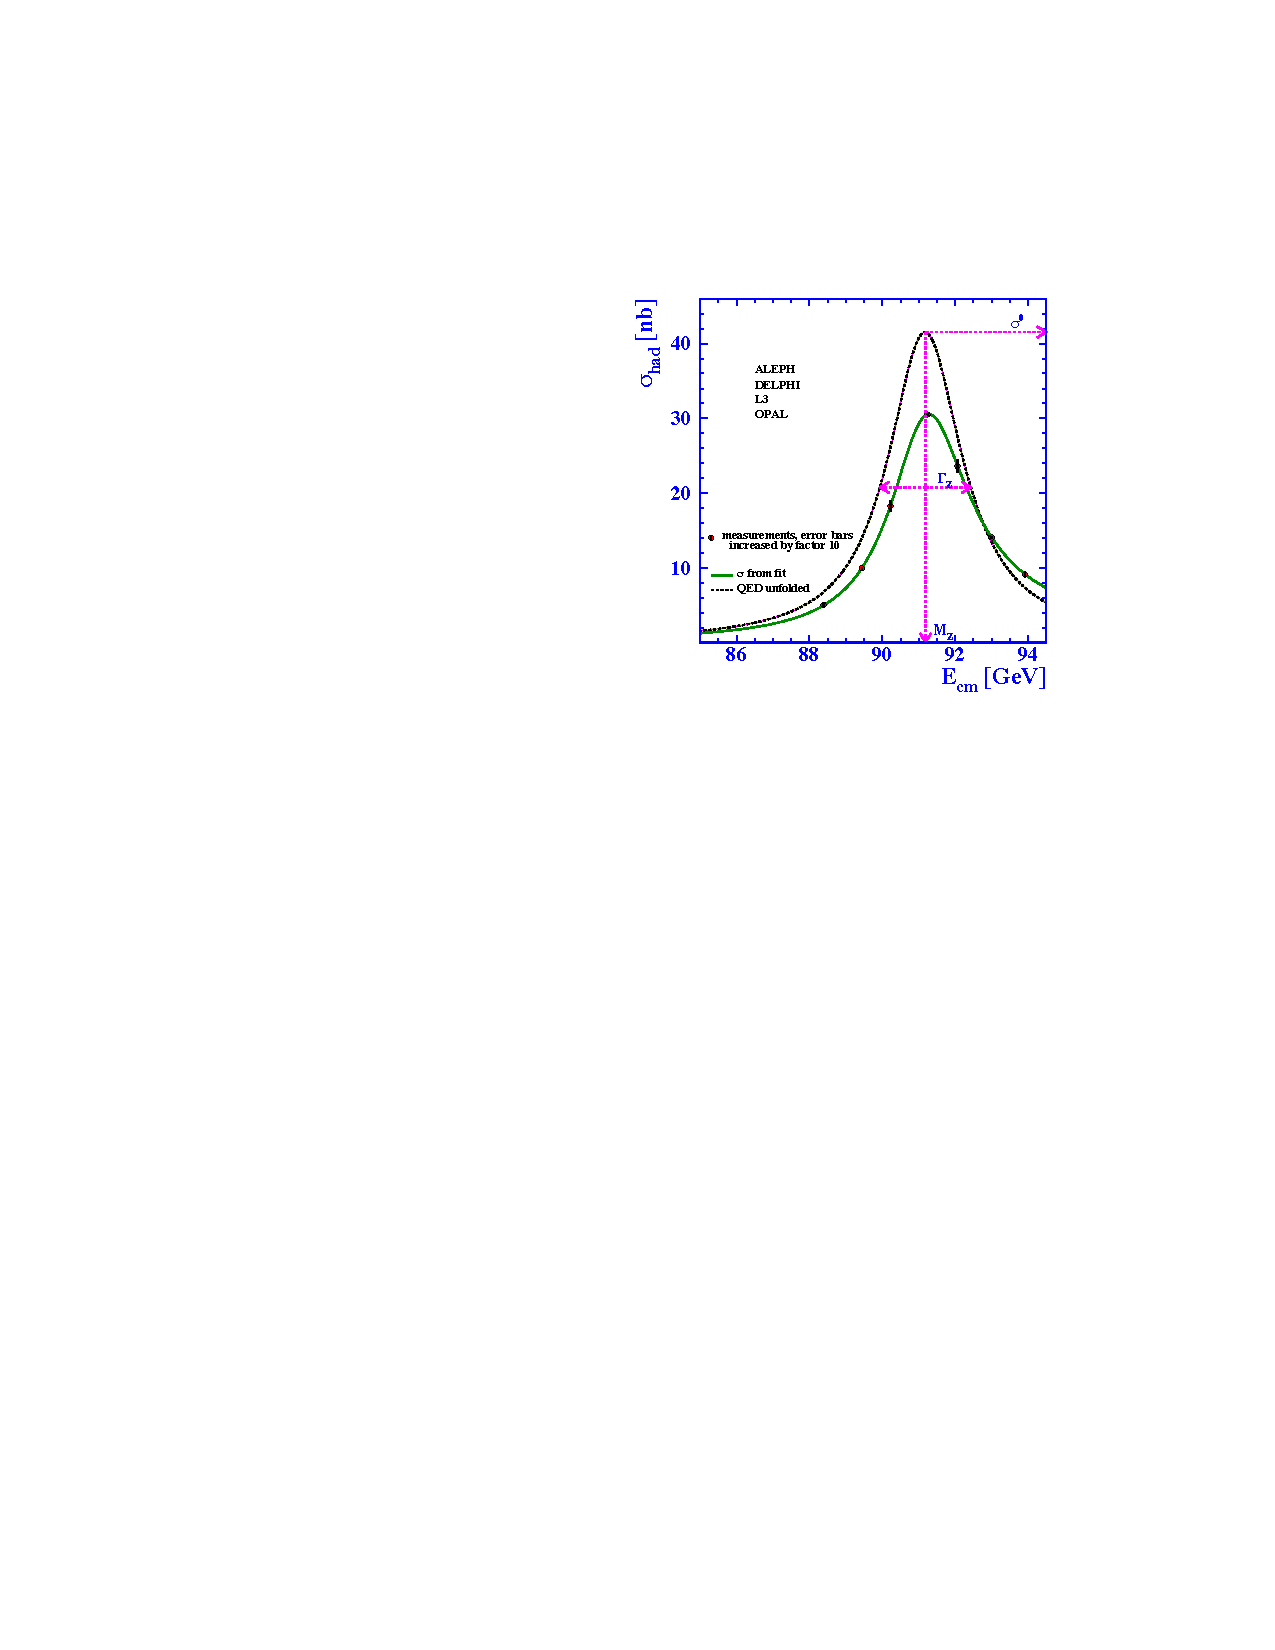
\includegraphics[scale=0.95]{LEP_hadronic_xsec}}
	\hspace{1cm}
	\subfloat[Measured and predicted dependence of the $q\overline{q}$, $\mu^{+}\mu^{-}$, and $\tau^{+}\tau^{-}$ pair production cross sections on LEP center-of-mass energy.]{\label{fig:LEP_pair_production_xsecs}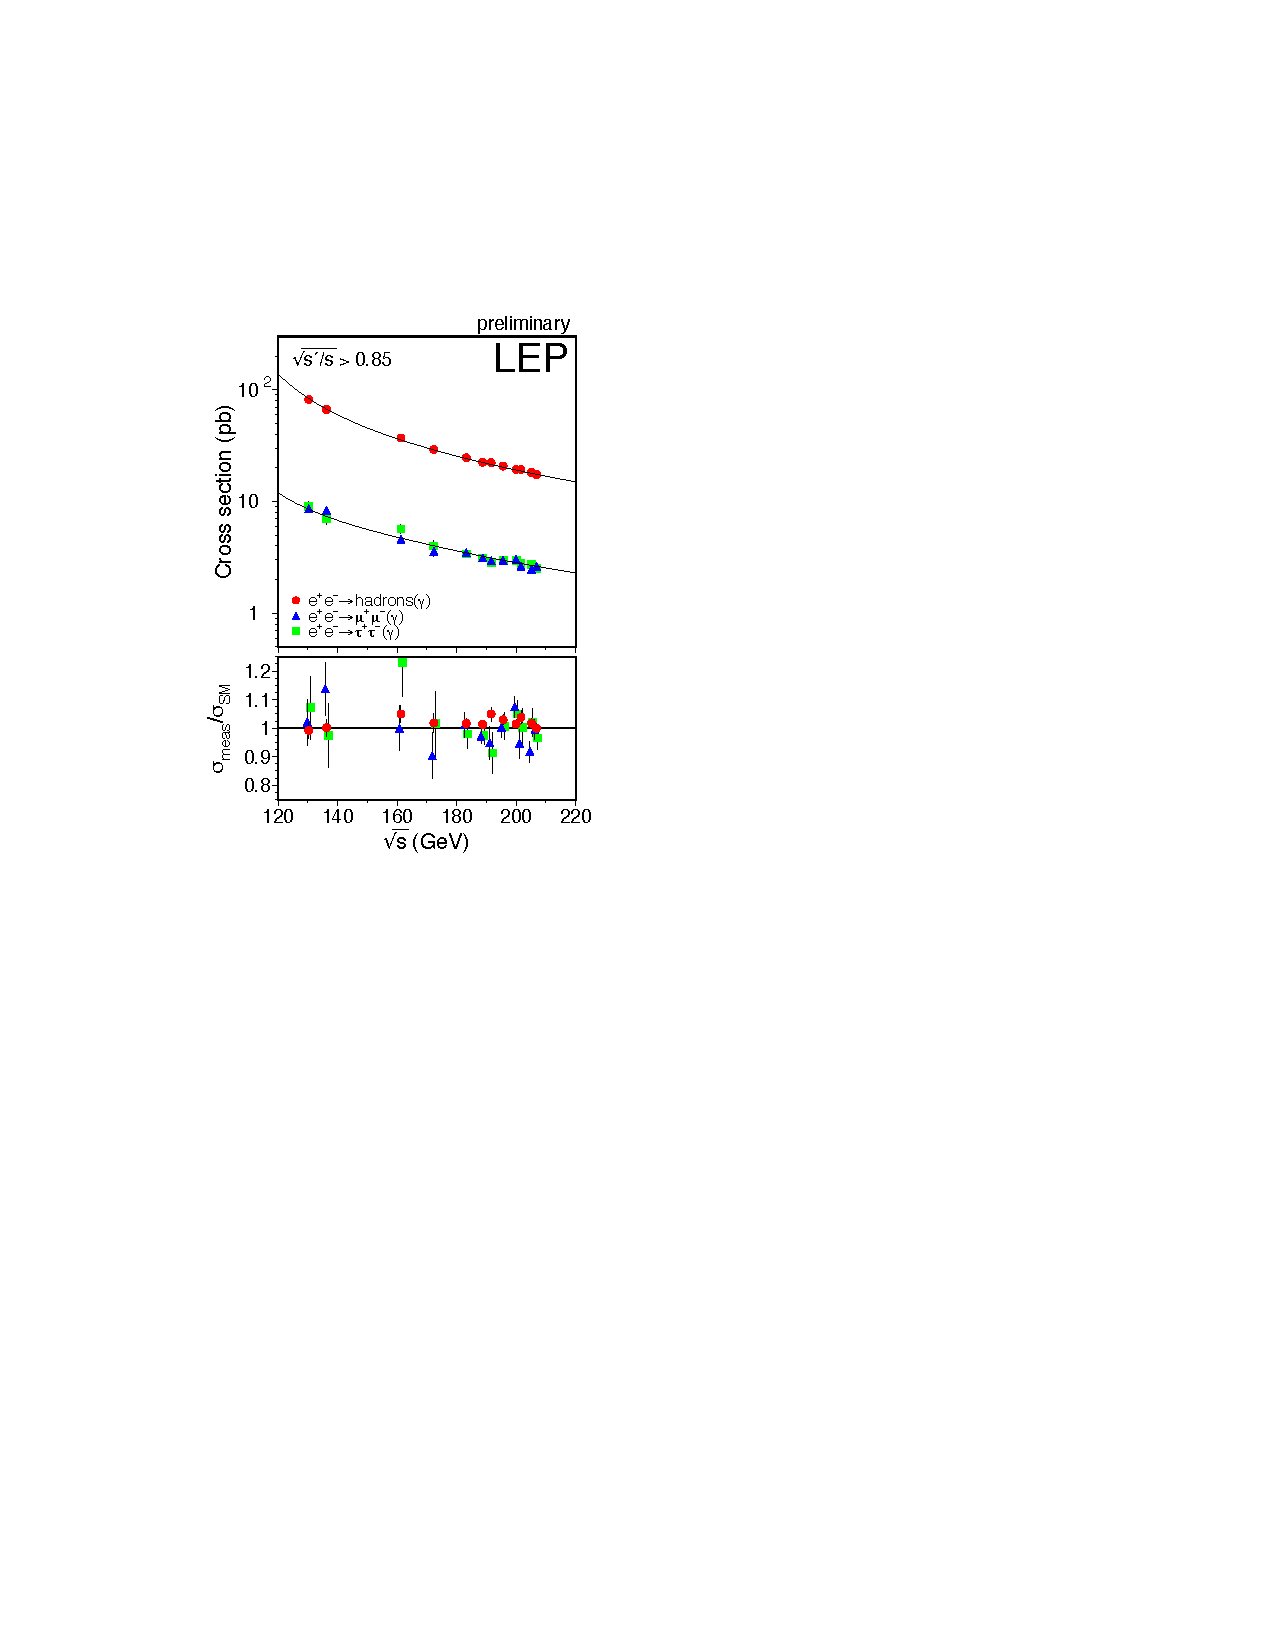
\includegraphics[scale=0.95]{LEP_pair_production_xsecs}}
	\\
	\subfloat[Measured and predicted dependence of the $W^{+}W^{-}$ pair production cross section on LEP center-of-mass energy.]{\label{fig:LEP_W_pair_production_xsec}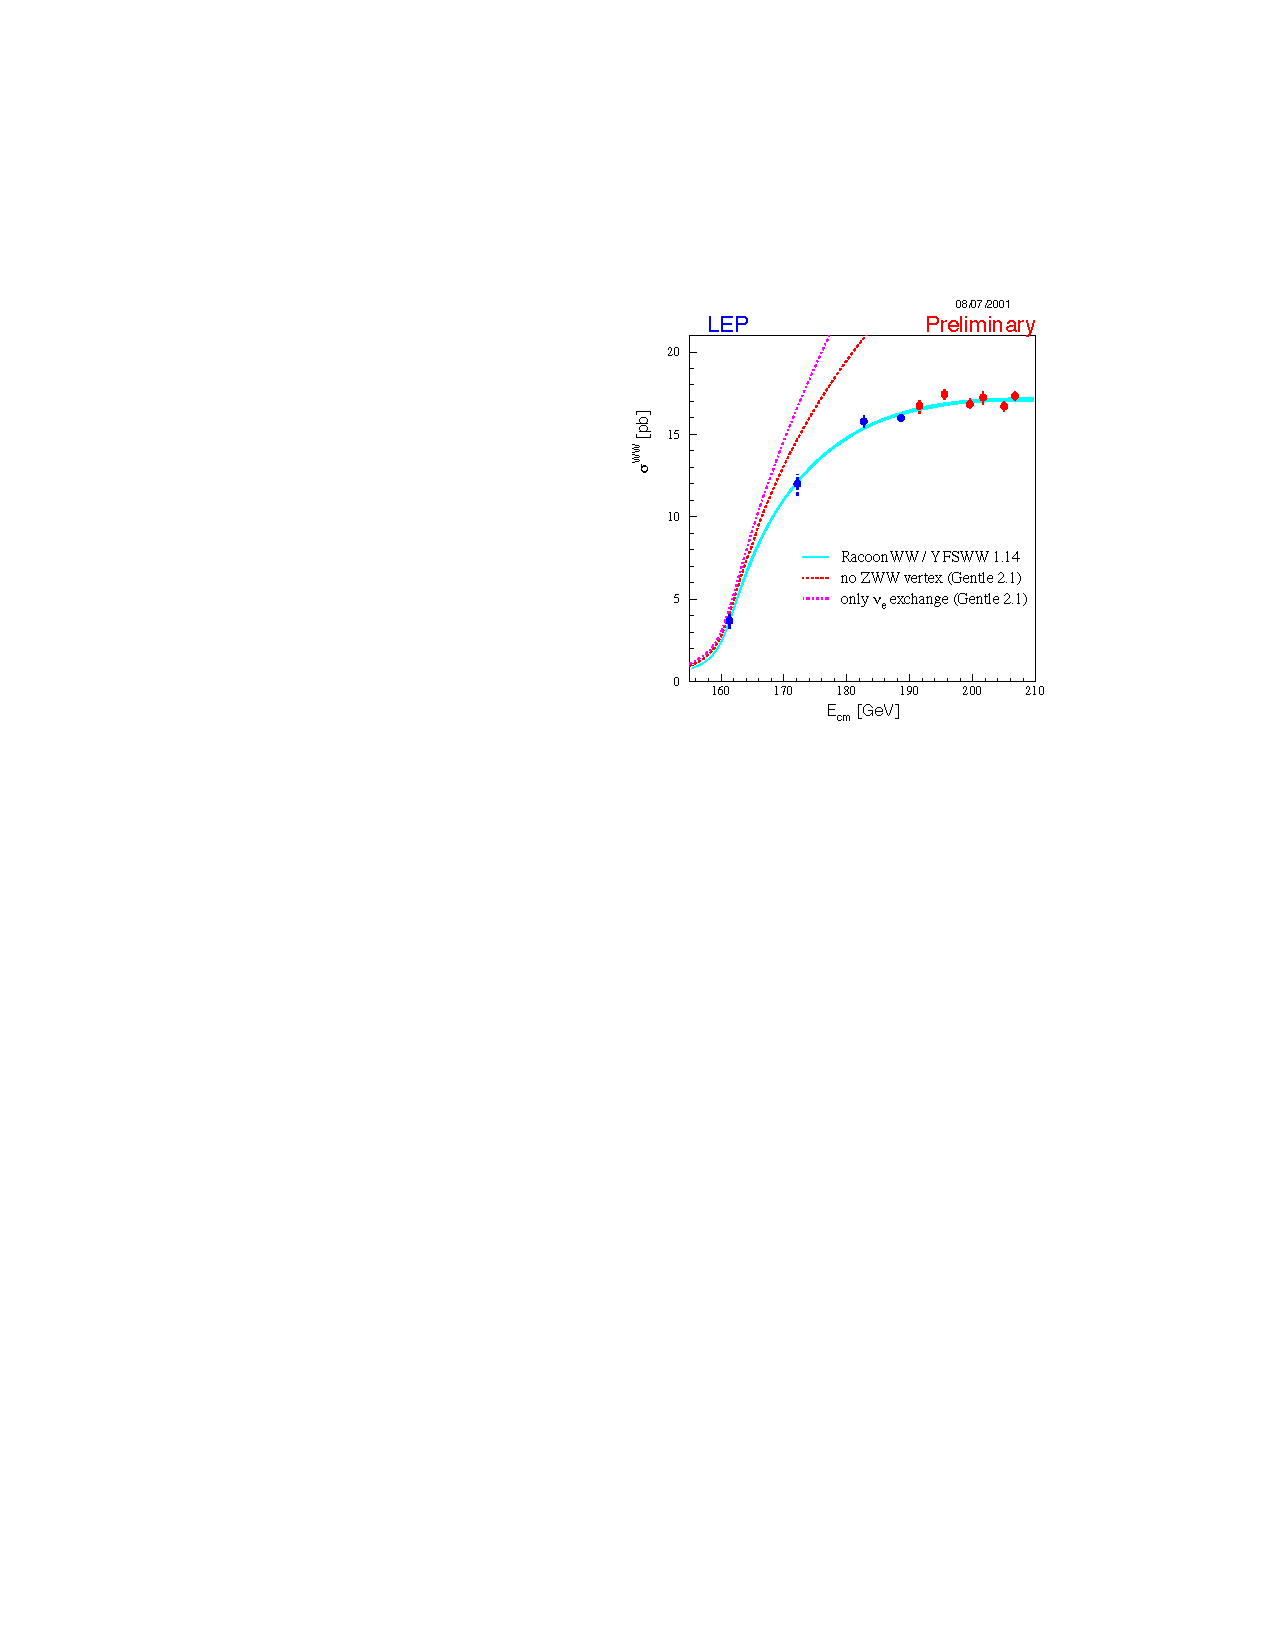
\includegraphics[scale=0.95]{LEP_W_pair_production_xsec}}
	\hspace{1cm}
	\subfloat[Measured and predicted dependence of the strong coupling constant $\alpha_{s}$ on LEP center-of-mass energy.]{\label{fig:LEP_alphaS_running}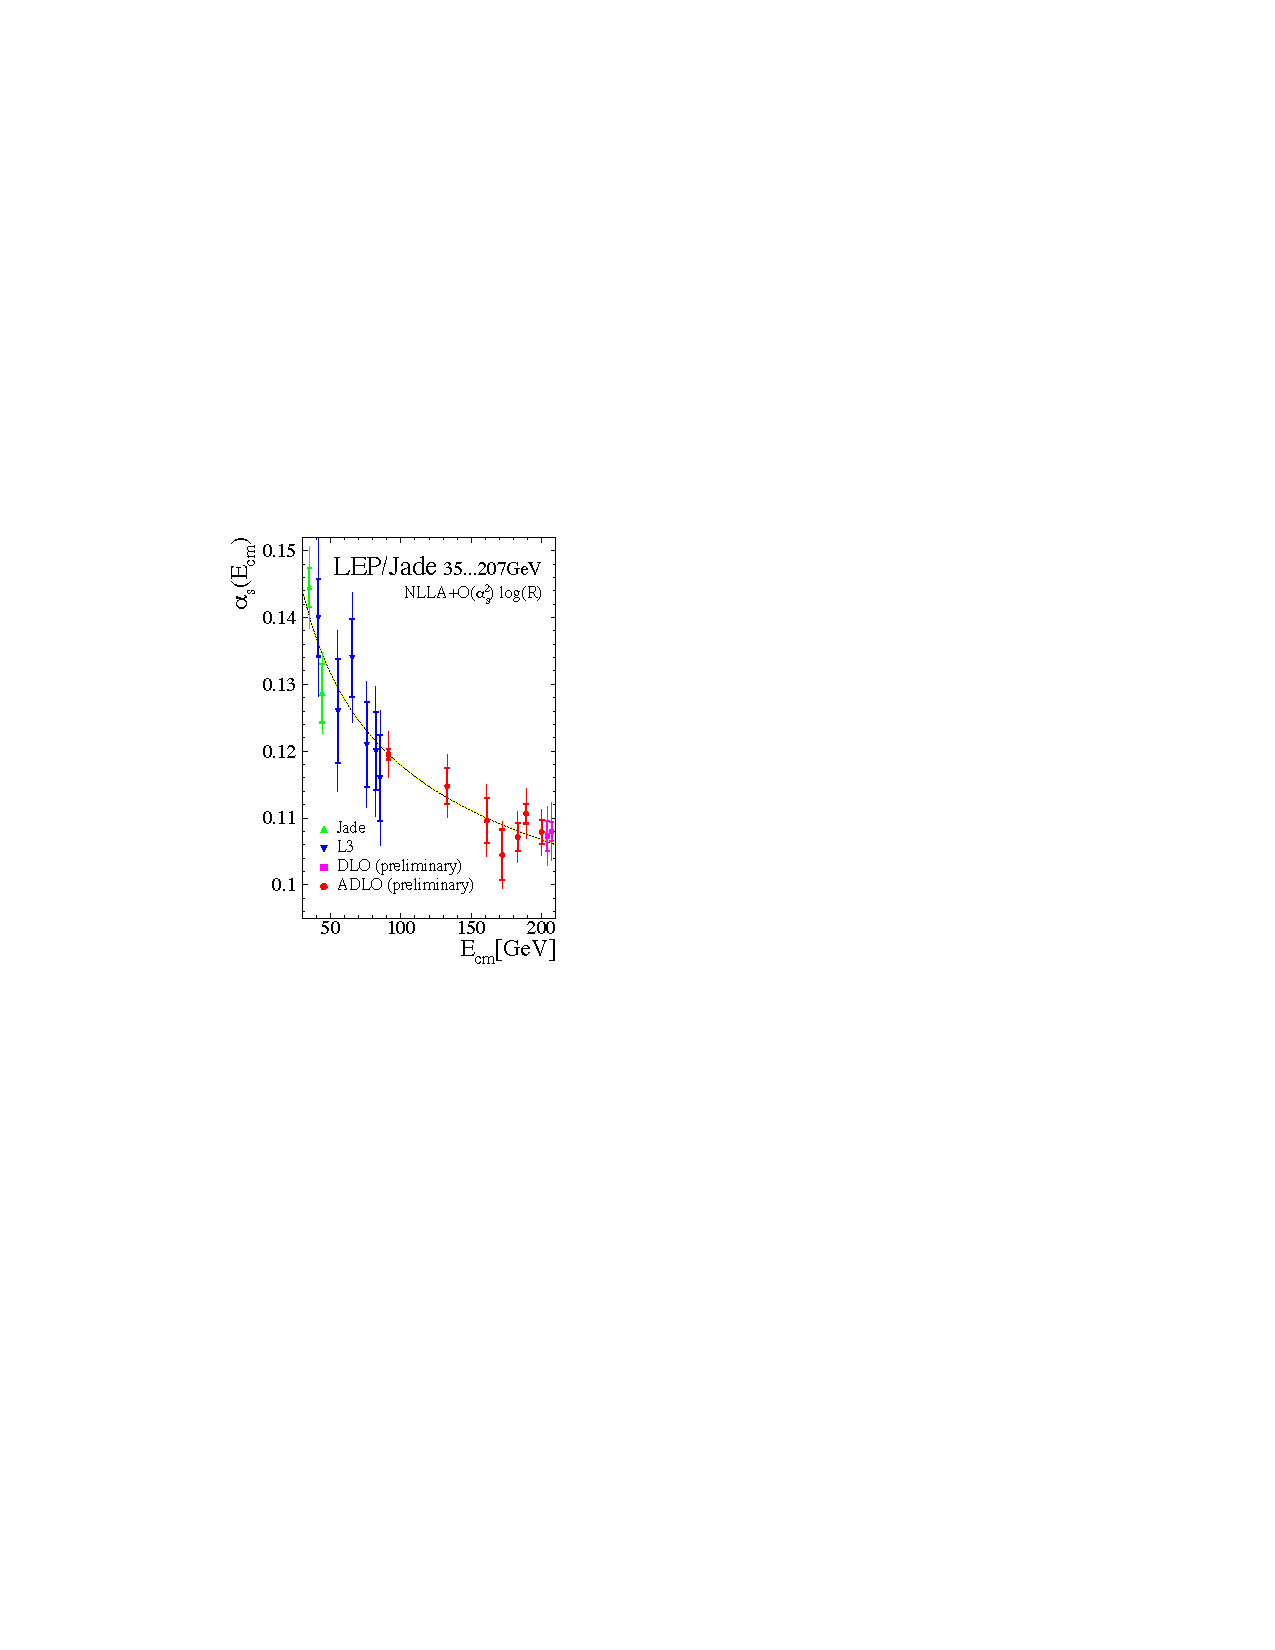
\includegraphics[scale=0.95]{LEP_alphaS_running}}
	\caption{Selected LEP measurements demonstrating its contribution to the precise understanding of the Standard Model.  Reprinted from ref. \cite{Drees}.}
	\label{fig:LEP}
\end{figure}

However, there are still deep problems with the Standard Model, stemming from the introduction of the Higgs scalar into the theory to break electroweak symmetry \cite{Higgs1964132,PhysRevLett.13.508,PhysRev.145.1156}.  Since the Higgs self-energy diagram diverges as the square of the ultraviolet cutoff scale, and assuming that there are no new important energy scales of physics between the weak scale ($\mathcal{O}$($10^{2}$ GeV/$c$)) and the Planck scale ($\mathcal{O}$($10^{19}$ GeV/$c$)), in order to be consistent with experimental measurements, this diagram must include a remarkable 17-orders-of-magnitude cancellation that is otherwise poorly motivated \cite{Aitchison:1111394}.  The quest to find new physics at an intermediate energy scale between the weak and Planck scales, and thus extend the Standard Model, was the driving force behind the construction of the Large Hadron Collider (LHC) in 2009, the world's highest energy particle accelerator to date.

Section~\ref{sec:The Standard Model and Electroweak Symmetry Breaking} of this chapter gives a brief overview of the Standard Model and electroweak symmetry breaking.  Sections~\ref{sec:Implications of the Higgs Mechanism} and~\ref{sec:Addressing Problems of the Standard Model with Supersymmetry} examine the issues raised by electroweak symmetry breaking that the Standard Model is as yet ill-prepared to address.

\section{The Standard Model and Electroweak Symmetry Breaking}
\label{sec:The Standard Model and Electroweak Symmetry Breaking}

All of the elementary matter particles (fermions)---quarks, charged leptons, and neutrinos---can be put in fundamental representations of the SM gauge groups.  The fermion content of the Standard Model is summarized in Table~\ref{tab:SM_particle_summary}.  The left-handed doublets are analogous to the spinors of non-relativistic quantum mechanics, with the $z$ component of ``weak isospin" $I_{3}$ equal to +1/2(-1/2) for the upper(lower) component of the doublet.

\begin{table}[htbp]
\caption{Fermion content of the Standard Model.  In the third column, the first number refers to the supermultiplet representation under $SU(3)_{C}$ (e.g. $\mathbf{3}$ means it has color charge and feels QCD), the second number refers to the representation under $SU(2)_{L}$ (e.g. $\mathbf{2}$ means it has weak isospin and feels the weak interaction), and the third number is the value of the hypercharge.  A bar over a number refers to the adjoint representation.  $\mathbf{1}$ means that the supermultiplet is not charged under that group, and thus does not feel the associated force (for example, the right-handed fermion singlets do not feel the weak interaction).}
\begin{minipage}{\textwidth}
\begin{tabular}{|l|c|m{5.5cm}|c|}
\hline
\multicolumn{1}{|c|}{Type} & Notation & Representation under $SU(3)_{C} \otimes SU(2)_{L} \otimes U(1)_{Y}$ & Couples to \\
\hline
\hline
\multirow{5}{*}{\begin{tabular}{@{}l@{}}Left-handed\\quark doublet\end{tabular}} & $\left(\begin{array}{c}u_{L} \\d_{L}\end{array}\right)$ & \multicolumn{1}{c|}{\multirow{5}{*}{($\mathbf{3}$, $\mathbf{2}$, $\frac{1}{6}$)}} & \multirow{5}{*}{$g$, $W$, $Z$, $\gamma$} \\
 & $\left(\begin{array}{c}c_{L} \\s_{L}\end{array}\right)$ & & \\
 & $\left(\begin{array}{c}b_{L} \\t_{L}\end{array}\right)$ & & \\
\hline
\multirow{3}{*}{\begin{tabular}{@{}l@{}}Right-handed\\up-type quark singlet\end{tabular}} & $u_{R}^{\dagger}$ & \multicolumn{1}{c|}{\multirow{3}{*}{($\mathbf{\bar{3}}$, $\mathbf{1}$, -$\frac{2}{3}$)}} & \multirow{3}{*}{$g$, $\gamma$} \\
 & $c_{R}^{\dagger}$ & & \\
 & $b_{R}^{\dagger}$ & & \\
\hline
\multirow{3}{*}{\begin{tabular}{@{}l@{}}Right-handed\\down-type quark singlet\end{tabular}} & $d_{R}^{\dagger}$ & \multicolumn{1}{c|}{\multirow{3}{*}{($\mathbf{\bar{3}}$, $\mathbf{1}$, $\frac{1}{3}$)}} & \multirow{3}{*}{$g$, $\gamma$} \\
 & $s_{R}^{\dagger}$ & & \\
 & $t_{R}^{\dagger}$ & & \\
\hline
\multirow{5}{*}{\begin{tabular}{@{}l@{}}Left-handed\\lepton doublet\end{tabular}} & $\left(\begin{array}{c}\bar{\nu}_{eL} \\e_{L}\end{array}\right)$ & \multicolumn{1}{c|}{\multirow{5}{*}{($\mathbf{1}$, $\mathbf{2}$, -$\frac{1}{2}$)}} & \multirow{5}{*}{$W$, $Z$, $\gamma$\footnote{Except for neutrinos, which have zero electric charge.}} \\
 & $\left(\begin{array}{c}\bar{\nu}_{\mu L} \\\mu_{L}\end{array}\right)$ & & \\
 & $\left(\begin{array}{c}\bar{\nu}_{\tau L} \\\tau_{L}\end{array}\right)$ & & \\
\hline
\multirow{3}{*}{\begin{tabular}{@{}l@{}}Right-handed\\charged lepton singlet\end{tabular}} & $e_{R}^{\dagger}$ & \multicolumn{1}{c|}{\multirow{3}{*}{($\mathbf{\bar{1}}$, $\mathbf{1}$, 1)}} & \multirow{3}{*}{$\gamma$} \\
 & $\mu_{R}^{\dagger}$ & & \\
 & $\tau_{R}^{\dagger}$ & & \\
\hline
\end{tabular}
\end{minipage}
\label{tab:SM_particle_summary}
\end{table}

There are two types of weak interactions: flavor-changing charged currents, in which an up-type and down-type quark or charged lepton and neutrino couple to a charged $W$, and neutral currents, in which a fermion couples to another of the same flavor and to a neutral $Z$.  The charged current interaction is maximally parity violating---it only couples left-handed fermion doublets.  The neutral current interaction has a term coupling left-handed doublets and a term coupling right-handed singlets.  There are no mass terms of the form $m_{f}^{2}(f_{L}\bar{f}_{R} + f_{R}\bar{f}_{L})$ in the electroweak part of the Lagrangian, as these would violate gauge invariance \cite{rosner2001flavor}.  The simplest way to link the left-handed and right-handed fermions is via a Yukawa interaction $-\xi\left[\bar{f}_{R}(\phi^{\dagger}f_{L}) + (\bar{f}_{L}\phi)f_{R}\right]$ where $\phi$ is a doublet of complex scalar fields \cite{rosner2001flavor}.

The fermion interaction part of the Lagrangian is \cite{rosner2001flavor}

\begin{eqnarray}
\mathcal{L}_{\mathrm{int}} &=& \bar{f}_{R}i\gamma^{\mu}(\partial_{\mu} + i\frac{g_{Y}}{2}A_{\mu}Y)f_{R} \nonumber \\
&&+\mbox{ }\bar{f}_{L}i\gamma^{\mu}(\partial_{\mu} + i\frac{g_{Y}}{2}A_{\mu}Y + i\frac{g_{L}}{2}\overrightarrow{\tau}\cdot\overrightarrow{b}_{\mu})f_{L}
\end{eqnarray}
%
where $g_{Y}$ and $g_{L}$ are the electromagnetic and weak coupling constants, respectively; $Y$ is the weak hypercharge; $A_{\mu}$ is the EM gauge field; $\overrightarrow{b}_{\mu}$ is a three-component vector of weak gauge fields; and $\overrightarrow{\tau}$ is a three-component vector of the three Pauli matrices.  Before electroweak symmetry breaking, the three weak gauge fields and the one EM gauge field are massless.  The three weak gauge fields correspond to the three generators (the Pauli matrices) of $SU(2)_{L}$.  The one EM gauge field corresponds to the one generator (the real scalar $Y$) of $U(1)_{Y}$, where $Y = 2(Q - I_{3})$ ($Q$ is electric charge).  For the $SU(3)_{C}$ part of the Lagrangian, there are eight massless gauge fields (the gluons) corresponding to the eight generators of $SU(3)_{C}$ (the Gell-Mann matrices).

To break the electroweak symmetry implicit in the massless gauge bosons, a doublet of complex scalar fields (the Higgs) is introduced.  It has a potential \cite{rosner2001flavor}

\begin{eqnarray}
V(\phi^{\dagger}\phi) &=& \mu^{2}\phi^{\dagger}\phi + |\lambda|(\phi^{\dagger}\phi)^{2}.
\label{eq:Higgs_potential}
\end{eqnarray}

Since $\mu^{2} < 0$, the potential has the shape of a sombrero, as shown in Figure~\ref{fig:Higgs_potential}.  At the minimum of the potential, the scalar fields are not zero, but have some positive vacuum expectation value (VEV) (it can be chosen such that one component is zero and the other is $\sqrt{-\mu^{2}/2|\lambda|}$).  Nature spontaneously chooses one of the infinitely many vacua along the circle of minimum $V$ in ($\Re\left[\phi\right]$, $\Im\left[\phi\right]$) space.

\begin{figure}
	\centering
	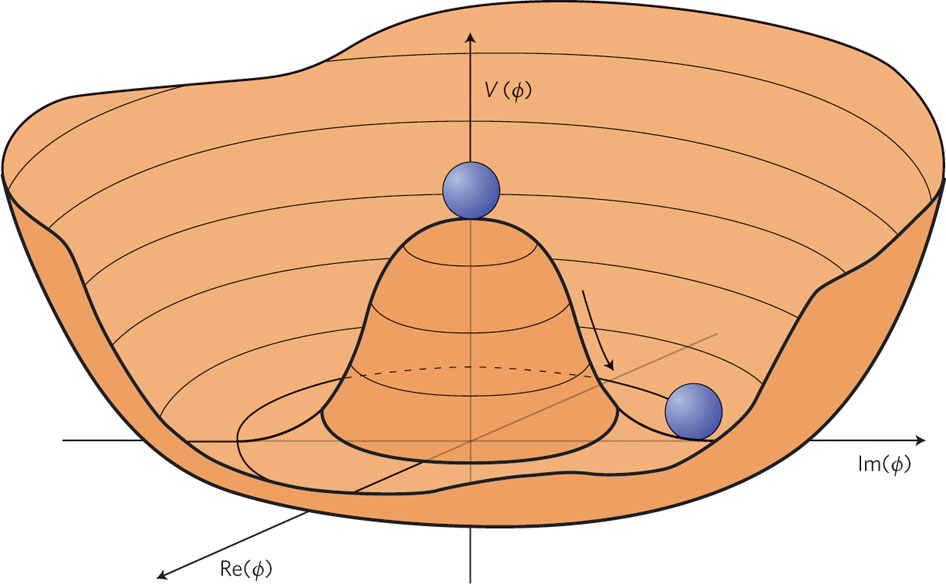
\includegraphics[scale=0.3]{Higgs_potential}
	\caption{Higgs potential (the sombrero) as a function of the real and imaginary parts of the complex scalar field.  The movement of the balls shows that the symmetry $\phi = 0$ is spontaneously broken, the stable vacuum state of nature being somewhere along the circle of minimum potential.  Reprinted from Fig. 1 of ref. \cite{Alvarez-Gaume}.}
	\label{fig:Higgs_potential}
\end{figure}

Expanding $\phi$ about its VEV $v$ in the Lagrangian introduces one massive scalar, the Higgs, and new mass terms for the gauge bosons.  However, the terms with positive mass are not the original $b_{1}$, $b_{2}$, $b_{3}$, and $A$ (spacetime indices dropped), but the observable $W^{\pm}$ and $Z^{0}$.  The $W^{\pm}$ are linear combinations of $b_{1}$ and $b_{2}$.  The $Z^{0}$ is one of the linear combinations of $b_{3}$ and $A$, the other being the massless photon $\gamma$.  After electroweak symmetry breaking (EWSB), the only remaining symmetry of the vacuum is electric charge, because the value of the electric charge operator acting on the Higgs VEV is zero.  As expected, there is one massless photon in the SM to reflect this symmetry.  The SM fermions can also acquire masses as a by-product of the Higgs mechanism via Yukawa terms.

\section{Implications of the Higgs Mechanism}
\label{sec:Implications of the Higgs Mechanism}

Before the formulation of the Higgs mechanism, physicists suspected that a heavy boson mediated the weak force from observations of $\beta$ decay, but had no way of putting a mass term into the Lagrangian without breaking gauge symmetry.  The Higgs mechanism of EWSB provided a way to generate masses for the $SU(2)_{L}$ gauge bosons.  Furthermore, it predicted the $W$ and $Z$ masses in terms of $g_{L}$, $g_{Y}$, and $v$.  $g_{L}$ and $g_{Y}$ could be measured in scattering experiments, and in 1983 the $W$ and $Z$ were first observed at the Super Proton-Antiproton Synchrotron (Sp$\bar{\mbox{p}}$S) at the European Organization for Nuclear Research (CERN) in Geneva, Switzerland \cite{Arnison:1983rp,Arnison1983398}.  Crucially, the values of the coupling constants and the gauge boson masses predict that the Higgs VEV should be 246 GeV, so the Higgs mass should not be too much different than that if $\lambda$ is to remain small enough to do perturbation theory \cite{Gunion:425736}.

The Higgs mechanism raises some interesting questions that cannot be immediately answered by SM physics.  First of all, why should $\mu^{2}$ be negative?  The form of the Higgs potential given in Eq.~\ref{eq:Higgs_potential} is about the simplest renormalizable form that can be written for a scalar field, but the choice of $\mu^{2} < 0$ is completely arbitrary.  Second, how can the hierarchy problem be avoided?

The Higgs mass squared receives one-loop corrections from all the particles it couples to; namely, all particles with mass.  Because the Higgs is a scalar particle, one-loop corrections are proportional to $\Lambda_{\mathrm{UV}}^{2}$, where $\Lambda_{\mathrm{UV}}$ is the ultraviolet cutoff energy of the loop integral.  $\Lambda_{\mathrm{UV}}$ can be interpreted as the energy at which the SM can no longer describe particle physics and non-SM physics takes over.  Ideally, $\Lambda_{\mathrm{UV}}$ is something like the Planck scale.  However, taking $\Lambda_{\mathrm{UV}} = M_{\mathrm{Planck}}$ implies that in order to keep the Higgs mass of order a few hundred GeV, as required by experimental tests of EWSB, a very large and precise counterterm must be applied at all orders in perturbation theory to the bare $m_{H}^{2}$.  The quadratic sensitivity of the Higgs mass to the cutoff scale and the extremely fine-tuned counterterms it necessitates is called the hierarchy problem.  SM fermions do not experience this problem because chiral symmetry prevents explicit fermion mass terms at any order, so by dimensional analysis, fermion masses can only be sensitive to $\ln\frac{\Lambda_{\mathrm{UV}}}{\Lambda_{\mathrm{other}}}$.

One of the most elegant ways to address these problems is to incorporate \textit{supersymmetry} (SUSY) into the SM.  Supersymmetry is new fundamental symmetry of nature between bosons and fermions, and will be discussed more thoroughly in Chapter~\ref{chap:The Supersymmetric Extension to the Standard Model}.  The next section just briefly describes how supersymmetry can mitigate some of the problems of the Higgs mechanism.

\section{Addressing Problems of the Standard Model with Supersymmetry}
\label{sec:Addressing Problems of the Standard Model with Supersymmetry}

As in the ordinary Standard Model, the couplings and masses in supersymmetric theory can be imposed at the supersymmetric scale and evolved down to the weak scale by use of renormalization group equations.  For many typical supersymmetric scenarios (like the one shown in Figure~\ref{fig:SUSY_RG_evolution}), $\mu^{2}$ is positive at the the supersymmetric scale but runs negative at the weak scale, leading to precisely the conditions needed for EWSB.  This is a consequence of the fact that the evolution of $m_{H}^{2}$ depends on the top quark Yukawa coupling, which, since the top is very heavy compared to the other quarks ($m_{t}\sim42m_{b}$, $m_{t}\sim136m_{c}$ \cite{0954-3899-37-7A-075021}), is large.  In some sense, then, supersymmetry not only provides the conditions for EWSB, but also explains why the top quark must be so much heavier than the other quarks.

\begin{figure}
	\centering
	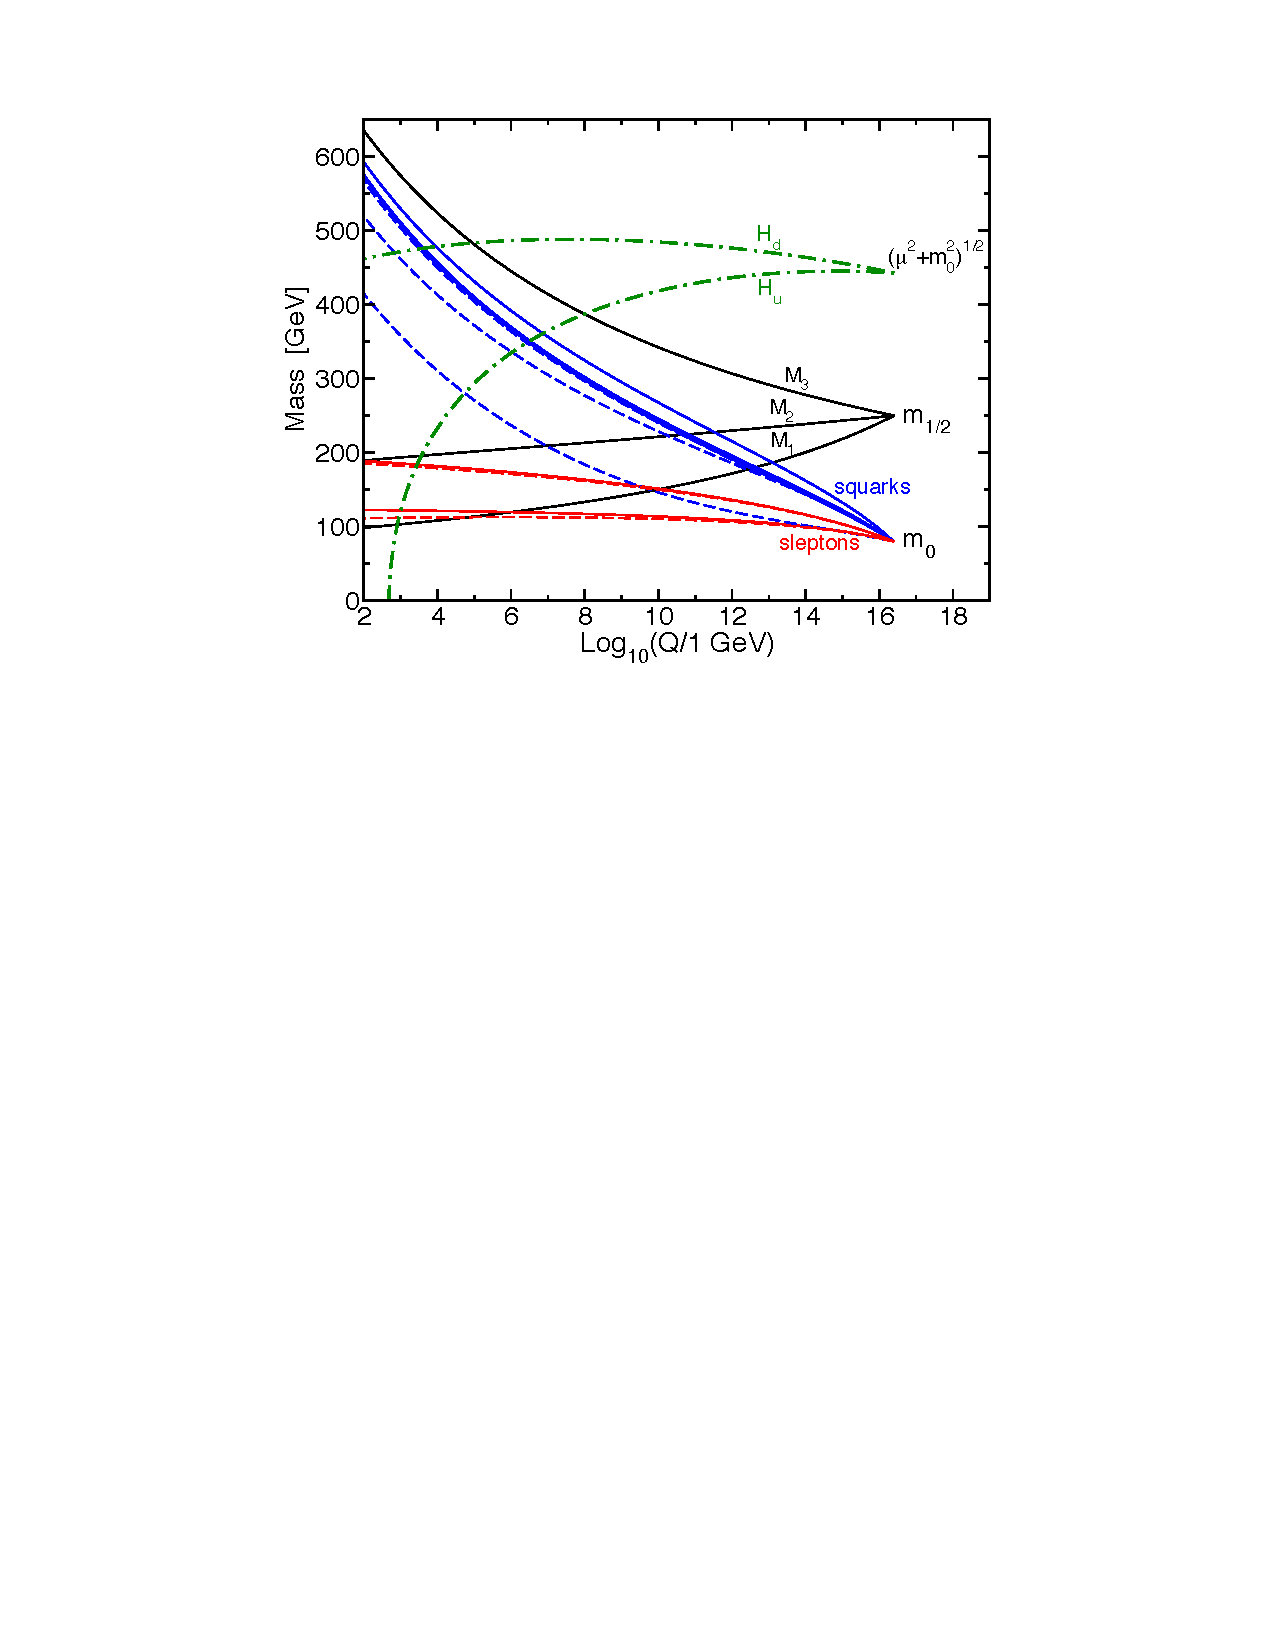
\includegraphics[scale=1.0]{SUSY_RG_evolution}
	\caption{Predicted evolution of the free parameters of supersymmetry as a function of renormalization scale for a representative set of SUSY parameters.  Note the dash-dotted line marked ``$H_{u}$" that goes negative at $\sim1$ TeV; this indicates $\mu^{2}$ running negative.  Reprinted from Fig. 7.4 of ref. \cite{SUSY_primer}.}
	\label{fig:SUSY_RG_evolution}
\end{figure}

SUSY's greatest strength, however, comes from the way it elegantly solves the hierarchy problem.  The Higgs squared mass corrections from fermion loops take the form \cite{SUSY_primer}

\begin{eqnarray}
\Delta m_{H}^{2} &=& -\frac{|\lambda_{F}|^{2}}{8\pi^{2}}\Lambda_{\mathrm{UV}}^{2} + ...
\label{eq:Higgs_mass_fermion_loop}
\end{eqnarray}
%
while the corrections from scalar loops would take the form \cite{SUSY_primer}

\begin{eqnarray}
\Delta m_{H}^{2} &=& \frac{|\lambda_{S}|^{2}}{16\pi^{2}}\Lambda_{\mathrm{UV}}^{2} + ...
\label{eq:Higgs_mass_scalar_loop}
\end{eqnarray}
%
where the ellipsis indicates terms proportional to $\ln\Lambda_{\mathrm{UV}}$ that do not pose a problem for the validity of the SM up to the Planck scale.  Since the fermion and scalar contributions have opposite signs, if each SM fermion were accompanied by two as-yet-undiscovered real scalar fields with $\lambda_{S} = |\lambda_{F}|^{2}$, then the problematic quadratic terms in Eqs.~\ref{eq:Higgs_mass_fermion_loop} and~\ref{eq:Higgs_mass_scalar_loop} would exactly cancel.  This is precisely the foundation of supersymmetry: for each fermion, there is a supersymmetric partner complex scalar boson.\footnote{The two real scalar fields combine to form one complex scalar field.}  This would remove the hierarchy problem altogether, and is the main reason physicists are eager to find evidence for the existence of supersymmetry at the LHC.

In addition to providing some rationale for the Higgs mechanism, SUSY makes two other very desirable predictions.  The first is that the strong, weak, and electromagnetic coupling constants will exactly unify at an energy scale of $10^{16}$ GeV/$c$, as shown in Figure~\ref{fig:SUSY_grand_unification}.  Unification of forces is not required by any experimental consideration, but is an elegant result nonetheless.  The second prediction of SUSY, explained in more detail in Sec.~\ref{sec:Phenomenology of General Gauge Mediation}, is the existence of a new stable and electrically neutral particle, undiscovered as of yet because of its extremely feeble (i.e. weak or gravitational) interactions with ordinary matter.  This particle might be what astronomers have observed as dark matter.  In fact, regardless of any theory, searches for evidence of dark matter at colliders are well motivated by suggestions from astronomy that some or all of the dark matter should have a mass at the weak scale \cite{Jungman1996195}.

\begin{figure}
	\centering
	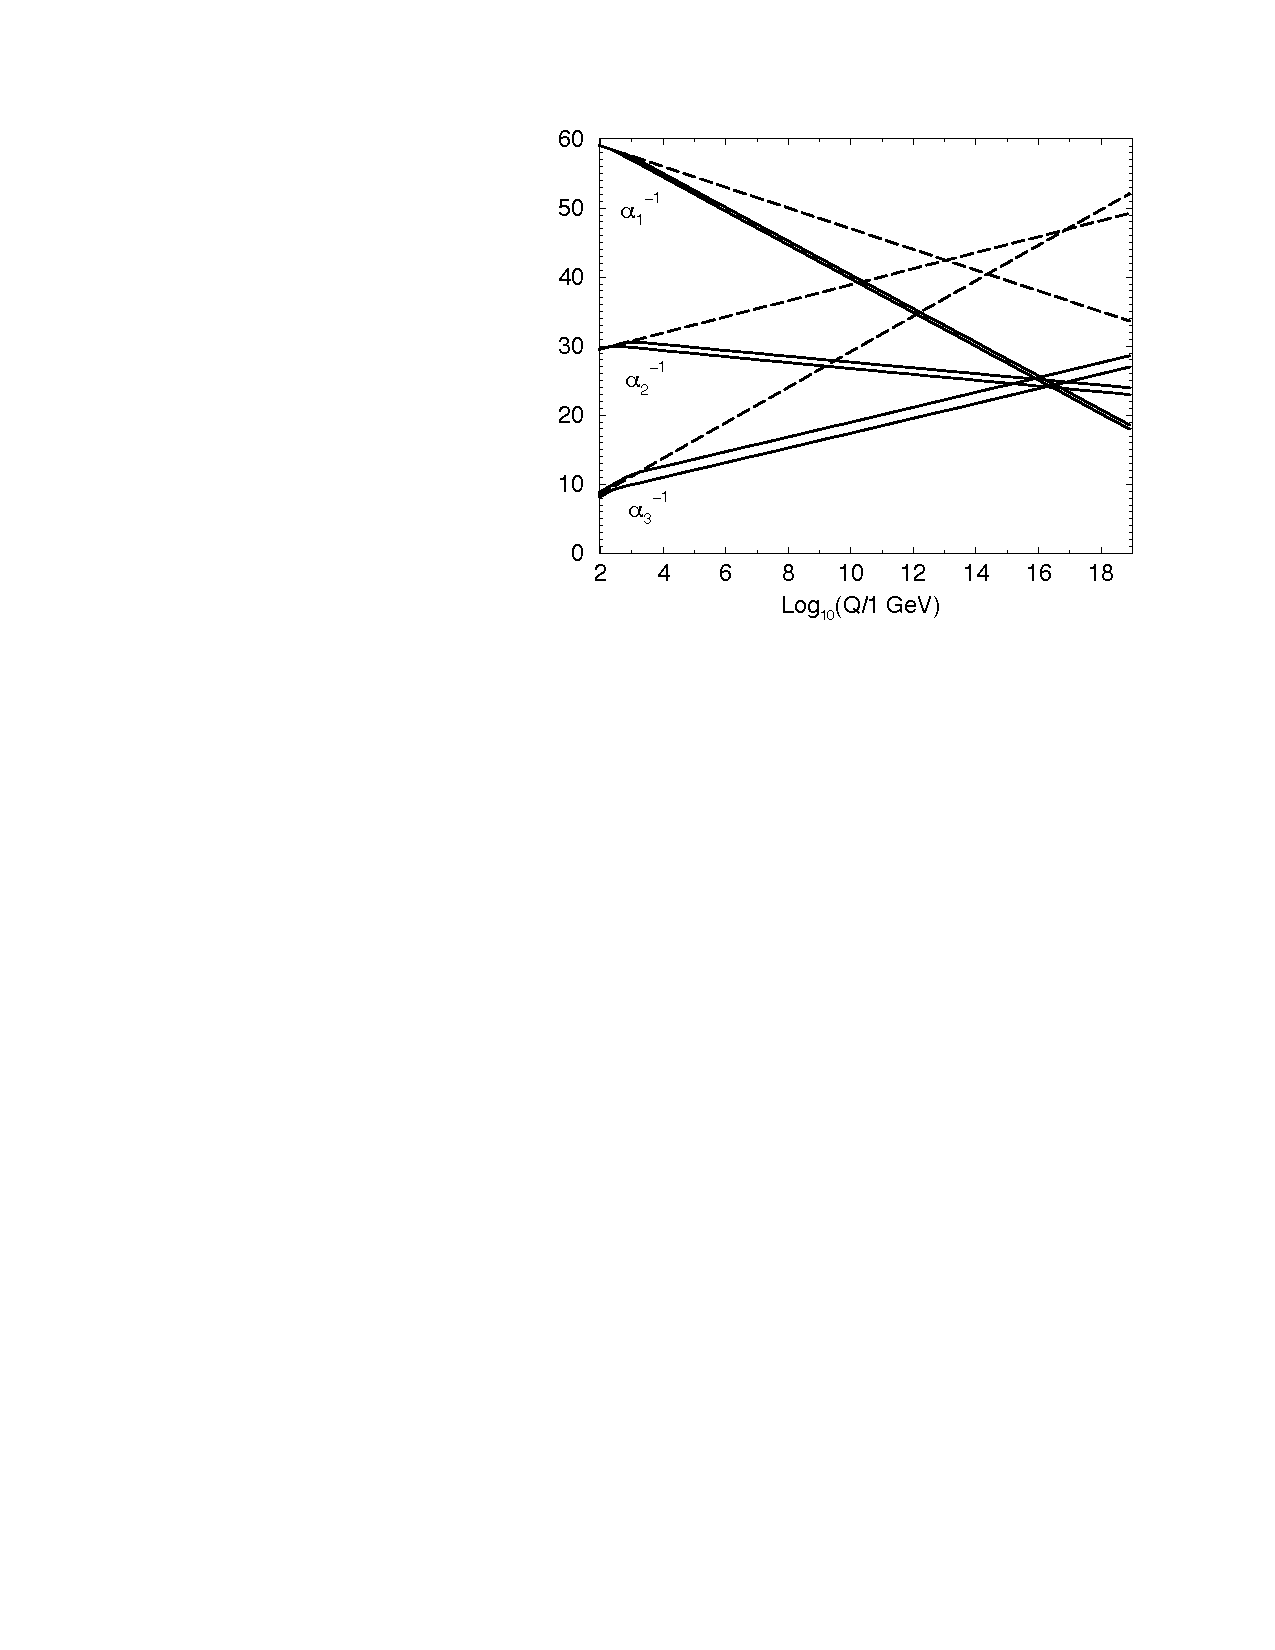
\includegraphics[scale=1.0]{SUSY_grand_unification}
	\caption{Inverse gauge couplings as a function of renormalization scale for the Standard Model assumption (dotted lines) and the SUSY assumption (solid lines; the double lines represent variations in SUSY parameters and in $\alpha_{S}(m_{Z})$).  Reprinted from Fig. 5.8 of ref. \cite{SUSY_primer}.}
	\label{fig:SUSY_grand_unification}
\end{figure}

Everything discussed in this chapter assumes that the Higgs mechanism is indeed the origin of EWSB.  It is important to remember that no experimental observation to date unequivocally establishes the existence of the Higgs scalar, although some activity recently unearthed in the LHC data \cite{Chatrchyan201226,Aad201249} tentatively suggest a Higgs mass of $\sim125$ GeV.  The discovery of the Higgs scalar would place an important restriction on the types of SUSY theories that might be consistent with experiment.  Operating at a 7 TeV center-of-mass energy, the LHC can thoroughly probe the scale of EWSB and the expected mass range of the Higgs, as well as the mass range of supersymmetric particles if SUSY is indeed the solution to the hierarchy problem and the light Higgs is found.  Therefore, discovering or excluding SUSY is a key goal of the LHC physics program.  The next chapter discusses SUSY more formally and shows what phenomenological consequences it entails.

\end{document}